\begin{figure}[htp]
\centering

\begin{minipage}{.45\textwidth}
    \centering
    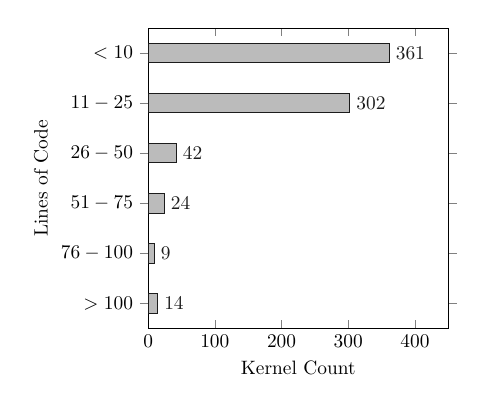
\begin{tikzpicture}[scale=0.7]
    
    \selectcolormodel{gray}
    
    \begin{axis}[
        xbar, xmin=0, xmax=450,
        xlabel={Kernel Count},
        symbolic y coords={
            {$> 100$},
            {$76-100$},
            {$51-75$},
            {$26-50$},
            {$11-25$},
            {$< 10$}
        },
        ytick=data,
        ylabel={Lines of Code},
        nodes near coords,
        nodes near coords align={horizontal},
        height=200pt, width=200pt
    ]
    
    \addplot coordinates {
        (14,{$> 100$})
        (9,{$76-100$})
        (24,{$51-75$})
        (42,{$26-50$})
        (302,{$11-25$})
        (361,{$< 10$})
    };
    
    \end{axis}
    \end{tikzpicture}
    
    \caption{Lines of Code}
    \label{Fi:code_lines}
\end{minipage}
\hfil
\begin{minipage}{.5\textwidth}
    \centering
    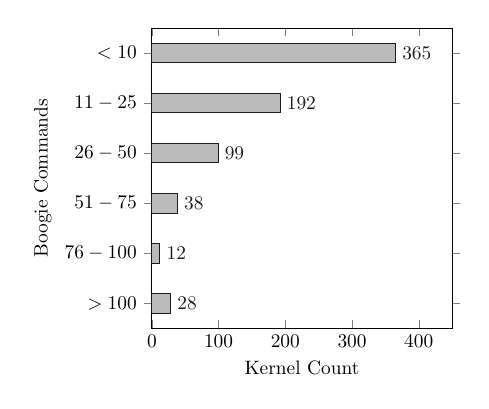
\begin{tikzpicture}[scale=0.7]
    
    \selectcolormodel{gray}
    
    \begin{axis}[
        xbar, xmin=0, xmax=450,
        xlabel={Kernel Count},
        symbolic y coords={
            {$> 100$},
            {$76-100$},
            {$51-75$},
            {$26-50$},
            {$11-25$},
            {$< 10$}
        },
        ytick=data,
        ylabel={Boogie Commands},
        nodes near coords,
        nodes near coords align={horizontal},
        height=200pt, width=200pt
    ]
    
    \addplot coordinates {
        (28,{$> 100$})
        (12,{$76-100$})
        (38,{$51-75$})
        (99,{$26-50$})
        (192,{$11-25$})
        (365,{$< 10$})
    };
    
    \end{axis}
    \end{tikzpicture}
    
    \caption{Boogie Commands}
    \label{Fi:boogie_commands}
\end{minipage}

\end{figure}
